
%%%%%%%%%%%%%%%%%%%%%%% file typeinst.tex %%%%%%%%%%%%%%%%%%%%%%%%%
%
% This is the LaTeX source for the instructions to authors using
% the LaTeX document class 'llncs.cls' for contributions to
% the Lecture Notes in Computer Sciences series.
% http://www.springer.com/lncs       Springer Heidelberg 2006/05/04
%
% It may be used as a template for your own input - copy it
% to a new file with a new name and use it as the basis
% for your article.
%
% NB: the document class 'llncs' has its own and detailed documentation, see
% ftp://ftp.springer.de/data/pubftp/pub/tex/latex/llncs/latex2e/llncsdoc.pdf
%
%%%%%%%%%%%%%%%%%%%%%%%%%%%%%%%%%%%%%%%%%%%%%%%%%%%%%%%%%%%%%%%%%%%


\documentclass[runningheads,a4paper]{llncs}

\usepackage{amssymb}
\setcounter{tocdepth}{3}
\usepackage{graphicx}
\usepackage{code}
\usepackage{hyperref}

\usepackage{url}
\urldef{\mailsa}\path|{alfred.hofmann, ursula.barth, ingrid.haas, frank.holzwarth,|
\urldef{\mailsb}\path|anna.kramer, leonie.kunz, christine.reiss, nicole.sator,|
\urldef{\mailsc}\path|erika.siebert-cole, peter.strasser, lncs}@springer.com|    
\newcommand{\keywords}[1]{\par\addvspace\baseelineskip
\noindent\keywordname\enspace\ignorespaces#1}
\newcommand{\comment}[1]{}

\begin{document}

\mainmatter  % start of an individual contribution

% first the title is needed
\title{A Little Language for Testing}

% a short form should be given in case it is too long for the running head
\titlerunning{A Little Language for Testing}

% the name(s) of the author(s) follow(s) next
%
% NB: Chinese authors should write their first names(s) in front of
% their surnames. This ensures that the names appear correctly in
% the running heads and the author index.
%
\author{Alex Groce \and Jervis Pinto}
%
\authorrunning{Alex Groce \and Jervis Pinto}
% (feature abused for this document to repeat the title also on left hand pages)

% the affiliations are given next; don't give your e-mail address
% unless you accept that it will be published
\institute{School of Electrical Engineering and Computer Science\\
Oregon State University, Corvallis, OR}

%
% NB: a more complex sample for affiliations and the mapping to the
% corresponding authors can be found in the file "llncs.dem"
% (search for the string "\mainmatter" where a contribution starts).
% "llncs.dem" accompanies the document class "llncs.cls".
%

\toctitle{A Little Language for Testing}
\tocauthor{Alex Groce and Jervis Pinto}
\maketitle


\begin{abstract}
The difficulty of writing test harnesses is a major obstacle to the
adoption of automated testing and model checking.  Languages designed
for harness definition are usually tied to a particular tool and
unfamiliar to programmers; moreover, such languages can limit
expressiveness.  Writing a harness directly in the language of the
software under test (SUT) makes it hard to change testing algorithms,
offers no support for the common testing idioms, and tends to
produce repetitive, hard-to-read code.  This makes harness
generation a natural fit for the use of an unusual kind of domain-specific language (DSL). This paper defines a \emph{template
scripting} testing language, TSTL, and shows how it can be used to
produce succinct, readable definitions of state spaces.  The concepts
underlying TSTL are demonstrated in Python but are not tied to it.


\end{abstract}


\section{Introduction}

Building a test harness is an often irksome task many users of formal
methods or automated testing face from time to time
\cite{woda08,woda12}.  The difficulty of harness generation is one
reason for the limited adoption of sophisticated testing and model
checking by the typical developer who writes unit tests.  This is
unfortunate, as even simple random testing can often uncover subtle
faults.

The ``natural'' way to write a test harness is as code in the language
of the Software Under Test (SUT).  This is obviously how most unit
tests are written, as witnessed by the proliferation of tools like
JUnit \cite{JUnit} and its imitators (e.g., PyUnit, HUnit, etc.).  It
is also how many industrial-strength random testing systems are
written \cite{ICSEDiff,AMAI}.  A KLEE ``test harness'' \cite{KLEE} for
symbolic execution is written in C, with a few additional constructs
to indicate which values are symbolic.  This approach is common in
model checking as well: e.g., Java Pathfinder \cite{JPF,JPF2} can
easily be seen as offering a way to define a state space using Java
itself as the modeling language, and CBMC \cite{CBMC,CBMCp} performs a
similar function in C, using SAT/SMT-based bounded model checking
instead of explicit-state execution.  JPF in particular has shown how
writing a harness in the SUT's own language can make it easy to
perform ``apples to apples'' comparisons of various testing/model
checking strategies \cite{JPFRandTest}.

\begin{figure}[t]
{\scriptsize
\begin{code}
op = choice(operations);
val1 = choice(values);
val2 = choice(values);
switch (op) \{
case op1:  if (guard1)
              call1(val1);
           break;
case op2:  if (guard2)
              call2(val1,val2);
           break;
case op3:  if (guard3)
              call3(val1,val3);
           break;
\end{code}
}
\vspace{-0.15in}
\caption {A test harness in the SUT language}
\label{fig:badharness}
\end{figure}



Unfortunately, writing test harnesses this way is a highly repetitive
and error-prone programming task, with many conceptual ``code clones''
(e.g. Figure \ref{fig:badharness}). A user faces difficult choices in
constructing such a harness. For example, the way guards and choices
are interleaved means that the state-space will be pointlessly
expanded to include many action and value choices that don't produce
any useful behavior.  This harness also always assigns {\tt val2} even
though {\tt call1} only uses {\tt val1}, to avoid having to repeat the
choice code for calls 2 and 3.  Moreover, this harness is possibly
sub-optimal for a method such as random testing, where the lack of any
memory for previously chosen values can make it hard to exercise code
behaviors that rely on providing the same arguments to multiple method
calls (e.g., {\tt insert} and {\tt delete} for container classes).
The construction of a harness becomes even more complex in realistic
cases, where the tested behaviors involve building up complex types as
inputs to method calls, rather than simple integer choices. For
example, consider the problem of testing or model checking a binomial
heap that supports several operations, defined in Figure
\ref{fig:binheap}.  Such a harness must manage the creation and
storage of values of multiple types, including heaps and references.
Moreover, because building up heaps and references is complicated,
they cannot simply be produced on each iteration, but must be
remembered.  As the interactions of multiple heaps (via {\tt union})
and references into a heap are the source of all interesting behavior,
the harness needs to decide how many heaps and references to store.
The code quickly becomes hard to read, hard to maintain, and hard to
debug.  In some cases \cite{AMAI} the code for a sophisticated test
harness approaches the SUT in complexity and even size!  The code's
structure also tends to lock in many choices (such as how to handle
storing heaps and references) that would ideally be configurable.

\begin{figure}[t]
{\scriptsize
\begin{code}
heap()                : returns a new heap
heap.insert(key,val)  : inserts a key with value, returning ref
heap.union(heap)      : merges two heaps
heap.extractMin()     : extracts the minimum
ref.delete()          : given a reference to a node, deletes it
ref.decreaseKey(key)  : decreases the key of ref's node
\end{code}
}
\vspace{-0.1in}
\caption{A binomial heap to test}
\label{fig:binheap}
\vspace{-0.20in}
\end{figure}

The definition of a harness also tends to be intimately tied to a
single tool, with the only testing strategies available being those
provided by that tool.  Writing novel testing strategies in even such
an extensible platform as Java Pathfinder is hardly a task for the
non-expert.
The harness in Figure \ref{fig:badharness} may support random testing and
some form of model checking, if it is written in Java and can use JPF
or a library for adaptation-based testing \cite{ISSRE12}. Such a
harness cannot support model checking or any sophisticated strategy
without being re-written if it is in a language like Python without
verification tool support.

What the user really wants is to simply provide the information in
Figure \ref{fig:binheap}, some configuration details (e.g., how many
{\tt ref}s to keep around), and some information on which testing
method to use (e.g., model checking, random testing, machine-learning
based approaches).  Some automated testing tools for Java \cite{FA11,Pacheco}
take a variation on this approach, automatically extracting the
signatures of methods from source code and testing them.
Unfortunately, completely automatic extraction often fails to handle
the subtle details of harness construction, such as defining guards
for some operations, or temporal constraints between API calls that
are not detectable by simple exception behavior.  The user wants
declarative harnesses, but often needs to program the details of a
harness.

\subsection{Domain Specific Languages for Testing}

The properties of the problem at hand suggest the use of a
\emph{domain-specific language} (DSL) \cite{ISOLA12}.  DSLs
\cite{Fow10} provide abstractions and notations to support a
particular programming domain. The use of DSLs is a formalization of
the long-standing approach of using ``little languages'' in computer
science, as memorably advocated by Jon Bentley in one of his famous
Programming Pearls columns \cite{LitLang} and exemplified in such system
designs as UNIX.  DSLs typically come in two forms: \emph{external}
and \emph{internal}.  An external DSL is a stand-alone language, with
its own syntax.  An internal DSL, also known as a domain-specific
embedded language (DSEL), is hosted in a full-featured programming
language, restricting it to the syntax (and semantics) of that
language.  Many attempts to define harnesses can be seen as internal
DSLs \cite{UDITA,ISSRE12,JPF2,CBMCp,KLEE}.  Neither of these choices
is quite right for harness definition.  Simply adding operations for
nondeterministic choice, as is done in most cases, still leaves most of
the tedious work of harness definition to the user, and makes changing
testing approaches difficult at best.  With an external DSL, the user
must learn a new language, and the easier it is to learn, the less
likely it is to support the full range of features needed.

A novel approach is taken in recent versions of the SPIN model checker
\cite{SPIN}.  Version 4.0 of SPIN \cite{ModelDriven} made use of
SPIN's nature as a tool that \emph{outputs a C program} to allow users
to include calls to the C language in their PROMELA models.  The
ability to directly call C code makes it much easier to model check
large, complex C programs \cite{AMAI,ModelCode}.  C serves as a
``DSEL'' for SPIN, except that, rather than having a domain-specific
language inside a general-purpose one, here the domain-specific
language hosts a general-purpose language.  A similar embedding is
used in {\tt where} clauses of the LogScope language for testing Mars
Science Laboratory software \cite{scriptstospecs}.  We adopt this
approach: embed a general-purpose language (for expressiveness) in a
DSL (for concision and ease-of-use).


\subsection{Template Scripting}

In previous discussions, a harness has been thought of as imperative
code that tests a system, even when the underlying use is more
declarative, as in CBMC, or as a purely declarative model stating the
available test operations, in which case the harness is often hidden
from the user and generated by a tool.  In this paper, we propose
thinking of a harness as a \emph{declaration of the possible actions
the SUT can take}, but where these actions are \emph{defined in the
language of the SUT itself, with the full power of the programming
language to define guards, perform pre-processing, and implement
oracles in an imperative fashion}.  Our particular approach is based
on what we call \emph{template scripting}.

The \emph{template} aspect is based on the fact that our method
proceeds by processing a harness definition file to output code in the
SUT's language for a test harness, much like SPIN.  The harness
description file consists of fragments of code in the SUT language
that are expanded, via code-generation, into executable source code.
The tool that outputs code basically defines a \emph{template} for
test harnesses in a programming language, and the harness definition
tells the tool how to instantiate that template.  Rather
than generating a testing tool, our method outputs \emph{a class
defining a search space}.  The \emph{scripting} aspect simply means
that our language is meant to be very lightweight, and assumes a host
language without a rigorous type system (e.g. Python) or with
effective type-inference (e.g. Scala), making minimal demands on the
user.  The design of the language also relies on the very-high-level
nature of code in scripting languages, making the harness concise but
expressive, and making ``one-liners'' of action definition possible.

\begin{figure}[t]
{\scriptsize
\begin{code}
@import bh

pool: \%INT\% 4
pool: \%HEAP\% 3
pool: \%REF\% 4

\%INT\%:=\%[1..20]\%
\%HEAP\%:=bh.heap()
\%REF\%:=\%HEAP\%.insert(\%INT\%,\%INT\%)
\%HEAP\%.insert(\%INT\%,\%INT\%)
\%HEAP\%.union(\%HEAP\%)
\%HEAP\%.extractMin()
\%REF\%.delete()
\%REF\%.decreaseKey(\%INT\%)
\end{code}
}
\vspace{-0.1in}
\caption{A simple harness definition for a binomial heap}
\vspace{-0.1in}
\label{fig:binheapharness}
\end{figure}

Figure \ref{fig:binheapharness} shows a complete harness definition
for the binomial heap class defined in Figure \ref{fig:binheap}.  The
example is easily understood by splitting it into three sections.
First, the single line proceeded by an ``@'' is raw Python, inserted
into the output harness with no modification in most cases.  This
section can be used not only to import the SUT's code, but to define
functions to be used in the body of the harness, as we will see below.
Second, the lines beginning with {\tt pool:} define the ``pool''
\cite{Pacheco,UDITA,AndrewsTR} of values that will be used during testing.  In
model checking terms, these store the state of the SUT.  There is no
type information here, because the template approach simply assumes
the type system of the host language, but in an informal sense each
pool value typically represents its own type in the template language,
as shown by its usage below (a pool value will correspond to inputs of
a particular type to method calls, in the most trivial instance, but
can also be used to encode more fine-grained type distinctions not
present in the host language).  The numbers indicate how many values
of a given pool ``type'' are needed.  Here, at least two {\tt INT}s
are needed, unless both values provided to {\tt insert} should always
be the same.  Similarly, there need to be at least two {\tt HEAP}s if
{\tt union} is to be tested effectively.  Because the performance of
random testing and some learning algorithms depends heavily on pool
sizes, we want to make it easy to experiment with them.  
%The use of
%pools to build up test elements is inspired by Randoop \cite{Pacheco},
%used in UDITA \cite{UDITA}, and aligned with the canonical form for
%unit tests defined by Andrews et al. \cite{AndrewsTR}.

Finally, the remainder of the harness definition simply gives possible
actions, one on each line.  Each line is expanded into Python code for
1) the actual test action represented and 2) a guard that determines
if that action is enabled, as shown in Figure \ref{fig:pybinheap}.
The functions for actions and guards are then added to a list that
stores all possible SUT actions, with no remaining nondeterminism
unless the SUT provides it.  Nondeterminism is controlled by choosing
which actions (whose guards are currently satisfied) to execute.  Even in the absence of user-defined guards, some
guards are automatically generated.  First, no \emph{uses} of a pool
value are allowed until that value has been assigned (the generated
harness initializes pool values as {\tt None}, a special Python
value).  Second, no pool value can be assigned to unless it is either
uninitialized or has been \emph{used} at least once.  This is critical
to avoid the potential for some test strategies (such as random
testing) to repeatedly perform useless assignments to values used in
the actual testing (e.g., {\tt INT[1] = 1} followed immediately by {\tt
  INT[1] = 2}.  Figure \ref{fig:validbinheaptest} shows an example of
a test that can be generated by this harness.  Note that assigning
anything to {\tt INT[3]}, {\tt REF[0]} or {\tt REF[1]} is not valid
after the final action of the test, as these pool values have been
assigned but not used.

\begin{figure}[t]
{\scriptsize
\begin{code}
import bh as b
class t(object):
   def act0(self):
      self.p\_INT[0]=1
      self.p\_INT\_used[0]=False
   def guard0(self):
      return (self.p\_INT\_used[0])
...
   def act87(self):
      self.p\_REF[0]=self.p\_HEAP[0].insert(self.p\_INT[1],self.p\_INT[0])

      self.p\_INT\_used[1]=True
      self.p\_INT\_used[0]=True
      self.p\_REF\_used[0]=False
      self.p\_HEAP\_used[0]=True
   def guard87(self):
      return (self.p\_INT[1] != None) and (self.p\_INT[0] != None) and
        (self.p\_REF\_used[0]) and (self.p\_HEAP[0] != None)
...
      self.actions.append((r"self.p\_INT[0]=1",self.guard0,self.act0))

\end{code}
}
\vspace{-0.15in}
\caption{Fragments of Python code for binomial heap harness}
\vspace{-0.1in}
\label{fig:pybinheap}
\end{figure}


\begin{figure}[t]
{\scriptsize
\begin{code}
self.p\_INT[1]=9
self.p\_INT[2]=1
self.p\_INT[0]=18
self.p\_HEAP[0]=b.heap()
self.p\_REF[2]=self.p\_HEAP[0].insert(self.p\_INT[0],self.p\_INT[2])
self.p\_INT[3]=17
self.p\_INT[0]=18
self.p\_REF[0]=self.p\_HEAP[0].insert(self.p\_INT[0],self.p\_INT[1])
self.p\_REF[0].decreaseKey(self.p\_INT[1])
self.p\_INT[1]=19
self.p\_REF[1]=self.p\_HEAP[0].insert(self.p\_INT[0],self.p\_INT[1])
self.p\_REF[0]=self.p\_HEAP[0].insert(self.p\_INT[0],self.p\_INT[1])
self.p\_HEAP[1]=b.heap()
self.p\_HEAP[1].union(self.p\_HEAP[0])
\end{code}
}
\caption{A valid action sequence (test) for the binomial heap harness}
\label{fig:validbinheaptest}
\end{figure}


\section{The Template Scripting Testing Language (TSTL)}

\begin{figure}[t]
{\scriptsize
\begin{code}
<template> ::= <template-line> EOL <template> | EOF
<template-line> ::= <raw> | <pool> | <property> | <init> | 
                    <feature> | <reference> | <compare> | <action>
<raw> ::= @ <raw-code>
<pool> ::= pool: \%<ID>\% <INT> [REF]
<property> ::= property: <simple-code>
<init> ::= init: <simple-code>
<feature> ::= feature: <regexp>
<reference> ::= reference: <regexp> ==> <text>
<compare> ::= compare: <regexp>
<action> ::= <text> | <lhs> := <rhs> | guardedFN(<simple-code>)
<raw-code> ::= <text> | def guardedFN(<text>) | \%COMMIT\%
<lhs> ::= <simple-code>
<rhs> ::= <simple-code>
<simple-code> ::= <text> | <simple-code> <ID-use> <simple-code> |
                  <simple-code> <range> <simple-code>
<ID-use> ::= \%<ID>\% | ~\%<ID>\%
<range> ::= \%[INT..INT]\%
\end{code}
}
\caption{The Template Scripting Testing Language in Pseudo-BNF}
\label{fig:corelang}
\end{figure}

\begin{table}[t]
\begin{tabular}{|l|l|l|}
\hline
Method & Type & Purpose \\
\hline
\hline
{\tt restart} & {\tt ()$\rightarrow$()} & resets pools, executes {\tt <init>} code\\
{\tt actions} & {\tt ()$\rightarrow$[(str,()$\rightarrow$bool,()$\rightarrow$())]} & returns a list of all possible actions \\
{\tt enabled} & {\tt ()$\rightarrow$[(str,()$\rightarrow$bool,()$\rightarrow$())]} & returns actions with True guard\\
{\tt check} & {\tt ()$\rightarrow$bool} & executes {\tt <property>} assertions \\
{\tt state} & {\tt ()$\rightarrow$STATE} & returns deep copy of pool values\\
%{\tt swarm} & {\tt ()$\rightarrow$[feature]} & disable a random set of features (returned as list)\\
{\tt replay} & {\tt [(str,()$\rightarrow$bool,()$\rightarrow$())] $\rightarrow$ bool} & replays a test, returns whether it failed \\
{\tt backtrack} & {\tt STATE$\rightarrow$()} & sets pools to STATE \\
%{\tt fails} & {\tt [(str,() $\rightarrow$ bool,()$\rightarrow$())] $\rightarrow$ bool} & returns True if the test fails \\
%{\tt reduce} & {\tt ([(str,()$\rightarrow$ bool,()$\rightarrow$())], [(str,()$\rightarrow$ bool,()$\rightarrow$())] $\rightarrow$ bool)} & returns a delta-debugged smaller test satisfying the predicate \\
%&  {\tt $\rightarrow$ [(str,()$\rightarrow$bool,()$\rightarrow$())]} & \\
\hline
\end{tabular}
\caption{SUT Class Methods}
\label{tab:sutmethods}
\vspace{-0.3in}
\end{table}

Figure \ref{fig:corelang} shows a BNF-style specification of the
Template Scripting Testing Language (TSTL).  Processing a harness
definition involves iterating through the lines in the file and
performing a set of transformations that result in an output file that
defines a class in the target language (Python in our current
implementation).  This class itself performs no testing; it instead
defines an interface to a definition of the available actions of the
SUT that any testing algorithm can use, shown in Table
\ref{tab:sutmethods}.\footnote{This is not the entire set of methods
TSTL compilation automatically generates: there are also methods for
swarm testing \cite{ISSTA12}, generalized delta-debugging \cite{DD,icst2014}, code coverage, and
other common testing needs.}  The methods in this interface are not
defined by the user, but automatically generated by the TSTL
``compilation.''  The basic transformation algorithm is relatively
simple (our implementation for Python is less than 1,000 lines of
code):

\begin{enumerate}
\item Output the {\tt <raw>} Python code, transforming guarded functions into expanded Python code as described in Section \ref{sec:guards}.
\item Collect the set of pool values, properties, initialization code, features, references, and comparisons.
\item Replace each pool ID in actions and properties with the pool ID plus a {\tt <range>} from 0 to the pool size - 1.  
\item Recursively expand each action and property range, creating copies with each value in the range instantiated.  At this point all actions should be deterministic\footnote{assuming the SUT itself is determinstic}
\item Collect assignments and uses from actions; assignments are IDs on the {\tt lhs} of a {\tt :=}; uses are IDs appearing in an action, such that ID is not an assignment or marked with a \textasciitilde.
\item Generate guards for each action:  first, ensure no values are used that have no value; second, ensure no assignments to values that have a value that has not  been used are made; third, add any guarded function calls as extra guards (see Section \ref{sec:guards}).
\item For any actions involving pools marked as {\tt ref},
copy with reference.
\item Apply all transformations indicated
by {\tt <reference>} (text matching {\tt regexp} is replaced by the
given {\tt text}), then add an assertion of equal return values for any
transformed code that matches a {\tt <compare>} regexp.
\item Perform any language-specific transformations.
\end{enumerate}

Due to lack of space here, we cannot elaborate on every aspect of
TSTL.  Instead, we present some example uses to highlight salient features.

\begin{figure}
{\scriptsize
\begin{code}
@def guardedAppend(l,item,limit):
@  if len(l) >= limit:
@    return False
@  %COMMIT%
@  l.append(item)

property: (len(%LIST%) < 10) or (6 not in %LIST%)
property: %VAL% != -1

pool: %LIST% 1
pool: %VAL% 1

%LIST% := []
guardedAppend(~%LIST%,%VAL%,10)
%VAL% := %[1..10]%
print %LIST%
\end{code}
}
\caption{A toy bounded list generation example ({\tt \%COMMIT\% } is expanded into a check for when the function is used as a guard) }
\label{fig:toylist}
%\vspace{-0.25in}
\end{figure}

\begin{figure}
{\scriptsize
\begin{code}
@import avl
@import bintree

pool: \%INT\% 4
pool: \%AVL\% 1 REF

\%INT\%:=\%[1..20]\%
\%AVL\%:=AvlTree()
\%AVL\%.insert(\%INT\%)
\%AVL\%.delete(\%INT\%)
\%AVL\%.find(\%INT\%)

reference: AvlTree() ==> BinTree()
compare: find

\end{code}
}
\caption{Using a reference as oracle}
\label{fig:binref}
\vspace{-0.25in}
\end{figure}

\subsection{Oracles}

TSTL handles test oracles in two ways.  First, users can specify
properties that the {\tt check} method will automatically verify using
assertion statements, expanded for each pool item involved.  Figure
\ref{fig:toylist} shows how properties are defined, in this case with
quite trivial properties.  Note that because raw Python can be used,
and properties can call arbitrary Python code, it is easy to encode
even complex specifications by defining a Python function that takes
the pool values of interest as input and returns a Boolean, then
adding it as a property.  A second popular approach to the oracle
problem is differential testing \cite{Differential}, also known as testing
with a reference.  TSTL supports this by making it easy to define how
to transform actions on the SUT into actions on the reference, and
when to compare values from calls to the SUT and reference.  Figure
\ref{fig:binref} shows a simple example, where an AVL tree in Python
is tested by comparing its behavior to a simple (unbalanced) binary
tree implementation.  All that is required to do this is 1) to mark
the AVL pool as a {\tt ref} pool, meaning it will have a copy that
contains a reference implementation 2) to explain how to transform the
call that initialized the AVL tree to initialize the binary tree and
3) to indicate that results from calling {\tt find} on the AVL and
reference should be compared.  TSTL automatically generates the required 
code based on this information.

\subsection{Guards and Function Calls}
\label{sec:guards}

As Figure \ref{fig:toylist} shows, TSTL makes it simple to define
functions and call them in actions.  Obviously, some actions cannot be
expressed as one line of code.  In these cases, we expect that the
user will define a function whose inputs can be any pool values, constants, etc. and perform more complex tasks.  We exploit this
feature to implement user-defined guards for actions easily.  If a
function is named {\tt guardedFN}, where {\tt FN} is a function name,
TSTL will automatically add an additional parameter to the function
definition when it generates a harness.  This parameter indicates
whether the call is to actually perform the action, or simply check if
the action is enabled.  The function definition should check the guard
and return {\tt False} if it is not satisfied.  At the point where the
user indicates that a ``real'' action is to follow (which typically modifies SUT state) the
function definition should include a {\tt \%COMMIT\%}, which will
be replaced with code that checks for a speculative call and simply
returns {\tt True} without proceeding if the call is in a guard
context.  The translation of the
relevant code from Figure \ref{fig:toylist} is shown in Figure
\ref{fig:toyexpand}, with a comment to indicate where the {\tt \%COMMIT\%} was.

\begin{figure}
{\scriptsize
\begin{code}
def guardedAppend(l,item,limit, SPECULATIVE\_CALL = False):
  if len(l) >= limit:
    return False
  if SPECULATIVE\_CALL: return True                                     \# /%COMMIT/%
  l.append(item)
...
   def act1(self):
      guardedAppend(self.p\_LIST[0],self.p\_VAL[0],10)

      self.p\_VAL\_used[0]=True
   def guard1(self):
      return (self.p\_LIST[0] != None) and (self.p\_VAL[0] != None) 
        and (guardedAppend(self.p\_LIST[0],self.p\_VAL[0],10,True))

\end{code}
}
\caption{User-defined guard example, Python code generated}
\label{fig:toyexpand}
\vspace{-0.15in}
\end{figure}

\subsection{Miscellaneous Notes on TSTL}

In order to effectively test the SUT, it is often important to build
up complex values before calling the code under test.  Making every
appearance of a pool element in an action a use, therefore allowing
the value to be reset to its initial state can ``suppress''
\cite{ISSRE13} behaviors, even if it does not strictly prevent them.
TSTL therefore allows the use of a \textasciitilde\ before a use of a
pool ID, as shown in Figure \ref{fig:toylist} to indicate that a
reference to a pool ID should not count as a use, it is simply
building up a complex input.  Another mitigation for suppression
effects is provided by the {\tt <feature>} definitions, which allow
TSTL to support swarm testing \cite{ISSTA12}.  Swarm testing is a
random testing approach in which each test disables some randomly
chosen API calls or grammar features, in order to better explore the
state space of the system.  A feature definition indicates that any
action matching the regexp is considered an instance of a certain
feature, and is disabled if that feature is disabled.  TSTL has strong out-of-the-box support for a variety of testing algorithms, some state-of-the-art like swarm testing.

\begin{figure}[t]
{\scriptsize
\begin{code}
@import sys
@import calculator as c
pool: %EXPR% 7
pool: %NUM% 5
%NUM% := '%[-100..100]%'
%NUM% := str(sys.maxint)
%NUM% := str(-sys.maxint - 1)
%EXPR% := %NUM%
~%EXPR% = '(' + ~%EXPR% + ')'
~%EXPR% = ~%EXPR% + '+' + ~%EXPR%
~%EXPR% = ~%EXPR% + '*' + ~%EXPR%
~%EXPR% = ~%EXPR% + '-' + ~%EXPR%
~%EXPR% = ~%EXPR% + '/' + ~%EXPR%
c.calculate(%EXPR%)
reference: c.calculate ==> eval
compare: calculate
\end{code}
}
\caption{Harness for a simple calculator class}
\label{fig:calc}
\end{figure}




Finally, we note that TSTL is not restricted to API testing.  Figure
\ref{fig:calc} demonstrates TSTL's support for encoding grammars for
generating strings.  It also provides an example of mixing
range values and explicit values in assignment.

\subsection{Output Language}

The language and tool presented here are not inherently tied to any
language.  With trivial modifications, the harness maker could output
Scala code instead of Python.  In principle, C or Java could also
serve as the base for the DSEL.  In fact, it should be simple to
output PROMELA models with embedded C, given a harness with C as the
base language, though maintaining the ``declarative'' approach would
make the PROMELA somewhat difficult to read (each SPIN
nondeterministic choice would need to pick the $n$th action, with the
guards being the enabled check).  Python was chosen for several
reasons: first, it is a widely adopted language in the real world,
particularly in the testing community.  Second, Python programs can
particularly benefit from more effective automated testing because the
lack of a good type system means Python code may
fail in surprising and frustrating ways.  

\section{Using the Harness to Test and Experiment}

\begin{figure}[t]
{\scriptsize
\begin{code}
t = SUT.t()
for ntests in xrange(1,config.maxtests+1):
    t.restart()
    test = []
    for s in xrange(0,config.depth):
        (name,guard,act) = random.choice(t.enabled())
        test.append(name)
        act()
	if not t.check():
            print "FAILED TEST:", test
            sys.exit(1)
print ntests, ``SUCCESSFUL''
\end{code}
}
\caption{A simple random tester}
\label{fig:randomtest}
\end{figure}

It is simpler to show how the interface described in Table
\ref{tab:sutmethods} is used than to explain each method.  Figure
\ref{fig:randomtest} shows the core of the implementation of a pure
random tester for an arbitrary SUT, omitting boilerplate such as
import statements, command-line option parsing, and checking for
timeout.  A few points are important: first, the test algorithm is
entirely SUT-agnostic.  All interaction with the SUT is performed through the API in Table \ref{tab:sutmethods}.  The use of pools and the {\tt (name, guard,
  action)} tuple list reduces the complex problem of choosing values and
operations as shown in Figure \ref{fig:badharness} to the uniform
simplicity of picking one enabled action and calling it as a function, storing the {\tt name} as a human-readable identifier for the test behavior.  Note that when reference oracles are used, the
call to {\tt act} is also typically enclosed in a {\tt try} block to
record the failing test, as is done with {\tt check}.


\begin{figure}
{\scriptsize
\begin{code}
t = SUT.t()
t.restart()
visited = []
S = []
S.append(t.state(), [])
test = []
while S != []:
    (v, test) = S.pop()
    t.backtrack(v)
    if (v not in visited) and (len(test) < config.maxdepth):
        visited.append(v)
        trans = t.enabled()
        for (name, guard, act) in trans:
            test.append(name)
            act()
            if not t.check():
                print "FAILED TEST:", test
                sys.exit(1)
            S.append((t.state(), test))
\end{code}
}
\caption{A really simple DFS-only model checker for safety properties}
\label{fig:modcheck}
\vspace{-0.25in}
\end{figure}

Perhaps more impressively, a natural consequence of encoding a state
space is that we can easily implement a (very simple) model checker,
as shown in Figure \ref{fig:modcheck}.  Of course, as a model checker
it is highly inefficient, since the visited check is implemented as a
linear search through a list of visited states.  The inefficient
linear search can be easily improved through the use of a hash table
for pool states.  TSTL makes use of Python's {\tt deepcopy}
functionality to automatically provide backtracking for many SUTs.  To
our knowledge, no other frameworks makes it as easy to use either
backtracking or replay for state restoration as TSTL. State copies are
often more efficient than replay.  However, for simple SUTs and
shallow depths replay may be better, and it works for some hard-to-copy
SUTs.

\begin{figure}
{\scriptsize
\begin{code}
t = SUT.t()

coverTool.clearCoverage()

for ntests in xrange(1, config.maxtests+1):
    t.restart()
    test = []
    print ntests+1, len(coverTool.getCoverage())
    for s in xrange(0,config.depth):
        possible = t.enabled()
        random.shuffle(possible)
        old = t.state()
        cov = coverTool.getCoverage()
	last = min(config.k, len(possible))
	pos = 0
        for (name, guard, act) in possible[:config.k]:
	    pos += 1
            test.append(name)
            act()
            if not t.check():
                print "FAILING TEST:", test
                sys.exit(1)
            covNew = coverTool.getCoverage()
            if (pos == last) or (len(covNew) > len(cov)):
                break
            coverTool.setCoverage(cov)
            t.backtrack(old)
\end{code}
}
\caption{A novel random testing algorithm, which is essentially random beam search, demonstrating the use of backtracking for state restoration}
\label{fig:novelrt}
\end{figure}

\begin{figure}
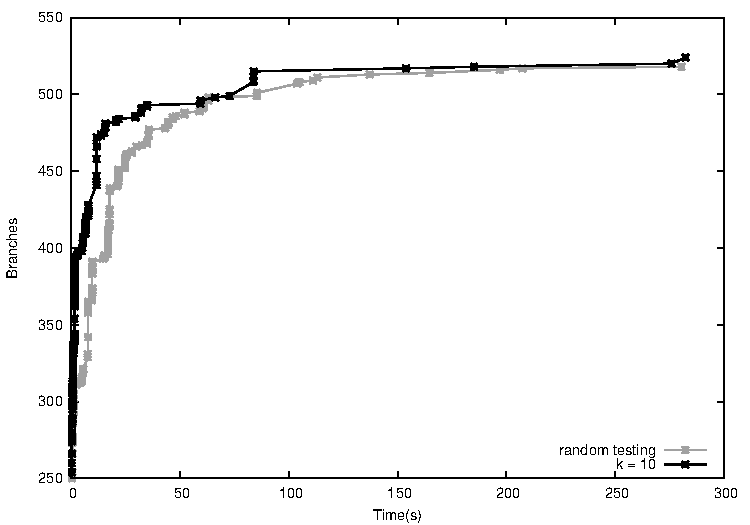
\includegraphics[width=4.2in]{explore}
\caption{Testing time vs. branches seen, traditional random testing vs. beam-search like method with $k=10$, for Dominion simulator}
\label{fig:explore}
\end{figure}

{\bf Exploring Novel Testing Algorithms:} In order to demonstrate how
TSTL facilitates the design and evaluation of testing approaches, we
provide the following simple algorithm motivated by classical beam
search.  Note that we do not claim this algorithm is highly effective
in general, the point is to show that it is extremely easy to
implement and compare new algorithms using TSTL.

Figure \ref{fig:novelrt} shows a modified random testing algorithm.
It performs almost like traditional random testing (as shown in Figure
\ref{fig:randomtest}) except for the following change: at each step of
the test, the state is saved.  Instead of randomly selecting a single
enabled action at random, this strategy picks $k$ actions at random,
and tries each one (backtracking to the old state after each action
but the final one).  However, if any action covers a
never-before-explored branch of the SUT, it is chosen and testing
proceeds to the next step immediately.\footnote{The coverage analysis
is provided in this example by a simple Python coverage
instrumentation tool, but TSTL offers integration with the very
popular {\tt coverage.py} as well.}  In less than thirty minutes, we
modified the random tester to perform this algorithm and both it and
the default random tester to output the time at which each new branch
is first covered during testing.  Figure \ref{fig:explore} shows the
branch discovery rate of random testing compared to the novel test
harness based on beam-search.  The SUT (an implementation of strategy
simulation for the card game Dominion) was taken from our work on
applying machine learning to test generation, where it had proven
difficult to improve on random testing.  The experiment shows that,
for this subject, the curve of covered code increases much more
rapidly using the modified beam search than with traditional random
testing.  This simple experiment shows the ease with which researchers
can explore novel testing strategies in TSTL.  The benefits of
providing backtracking are also evident here --- other experiments
show the same algorithm using replay performs considerably worse on
average, at the test lengths required for good code coverage.

\vspace{-0.1in}

\section{Related Work}


To our knowledge, there has been no previous proposal of a concise
\emph{language} like TSTL to assist users in building test
harnesses.  One line of related work is our own previous work on
building common frameworks for random testing and model checking
\cite{woda08} and proposing common terminology for imperative
harnesses \cite{woda12}.  Work on
domain-specific languages also informed our approach \cite{Fow10}.

There exist various testing tools and languages of a somewhat
different flavor: e.g. Korat \cite{Korat}, which has a much more fixed
input domain specification, or the tools built to support the Next
Generation Air Transportation System (NextGen) software
\cite{TameInputs}.  The closest of these is the UDITA language
\cite{UDITA}, an extension of Java with non-deterministic choice
operators and {\tt assume}, which yields a very different language
that shares our goal.  TSTL aims more at the \emph{generation} of
tests than the \emph{filtering} of tests (as defined in the UDITA
paper), while UDITA supports both approaches.  This goal of UDITA (and
resulting need for first-class {\tt assume}) means that it is hosted
inside a complex (and sometimes non-trivial to install/use) tool, JPF
\cite{JPF2}, rather than generating a stand-alone simple interface to
a test space, as with TSTL.  Building ``UDITA'' for a new language is
far more challenging than porting TSTL.  UDITA also supports far fewer
constructs to assist test harness development.

The design of the SPIN model checker \cite{SPIN} and its model-driven
extension to include native C code \cite{ModelDriven} inspired our
flavor of domain-specific language, though our approach is more
declarative than the ``imperative'' model checker produced by SPIN.
Similarly, work at JPL on languages for analyzing spacecraft telemetry
logs in testing \cite{scriptstospecs} provided a working example of a
Python-based declarative language for testing purposes.  The pool
approach to test case construction is derived from work on canonical
forms and enumeration of unit tests \cite{AndrewsTR}.

\section{Conclusions and Future Work}

We believe that the little language defined in this paper could be of
considerable use to software developers who would like to use more
automated testing, but do not want to learn complex new languages and
tools.  We expect that it also will prove useful to researchers who
would like to rapidly prototype new testing and model checking methods
and easily try their ideas out on new SUTs.  The use of a template
language makes it easy to exploit the usability of a scripting
language, and the declarative approach makes implementing new
testing algorithms easy.

Our future work is to further develop the TSTL language and tool,
based on other users' experiences.  One goal is to make use of TSTL
easy out-of-the-box, which means including many example harnesses,
SUTs, and testing algorithms.  A second task is to improve the core
language to include more functionality.  For example, one obvious
language omission is the inability to express desired probabilities
for random testing.  More automatic ranges, or a shorthand for
including multiple concrete values as choices on one line for grammar
encoding would also be useful.  We also plan to extend TSTL to handle
more host languages, including Scala, Java, C (possibly including use
of KLEE \cite{KLEE}), and PROMELA.  Additionally, we plan to use TSTL
as a basis for further research in using machine learning techniques
to improve software testing \cite{ISOLA12}.  A development version of
TSTL is available at \url{https://github.com/agroce/tstl}.

{\bf Acknowledgments:} The authors would like to thank Klaus Havelund,
Gerard Holzmann, Rajeev Joshi, John Regehr, Alan Fern, Martin Erwig,
and the anonymous NFM'15 reviewers for their comments and ideas.  A
portion of this research was funded by NSF CCF-1217824 and NSF
CCF-1054876.

\bibliographystyle{splncs03}

\bibliography{bibliography}

\end{document}
